\chapter{Background}\label{chapter:background}


\section{Definitions}

\paragraph{Strings.}

Let $\Sigma = \set{1, \dotsc, \sigma}$ be an \emph{alphabet} of size $\sigma$. A \emph{string} $S = S[1,n]$ over alphabet $\Sigma$ is a \emph{sequence} of \emph{characters} $S[1] \dotsm S[n]$, where $S[i] \in \Sigma$ for all $i$. For any string $S[1,n]$, we write $\abs{S} = n$ to denote its length. A \emph{substring} of $S$ is written as $S[i,j] = S[i] \dotsm S[j]$. Important types of substrings include \emph{prefixes} $S[1,j]$ and \emph{suffixes} $S[i,n]$. The concatenation of two strings $S[1,n]$ and $S'[1,n']$ is written as $SS' = S[1] \dotsm S[n] S'[1] \dotsm S'[n']$.

We define the \emph{lexicographic order} $<$ among strings in the usual way. For any two strings $S[1,n]$ and $S'[1,n']$, we have $S < S'$, if either $S[1] < S'[1]$ or $S[1] = S'[1]$ and $S[2,n] < S'[2,n']$. The \emph{empty string} $\lambda$ of length $0$ is a special case, with $\lambda < S$ for any non-empty string $S$ of length $\abs{S} > 0$. To avoid this special case, we often consider \emph{text} strings $T = T[1,n]$ that are terminated by an end marker $T[n] = \$ \not\in \Sigma$ with lexicographic value $0$. The \emph{lexicographic rank} of string $S$ among a collection (set) of strings $\mathcal{C}$ is the number of strings $S' \in \mathcal{C}$ such that $S' < S$, plus one. We often write $\mrank(T, S)$ to denote the lexicographic rank of string $S$ among all suffixes of text $T$, and $\mrank(\mathcal{C}, S)$ to denote the lexicographic rank of $S$ among the suffixes of all strings of collection $\mathcal{C}$.

The (Levenshtein) \emph{edit distance} between two strings $S$ and $S'$ is the minimum number of edit operations required to transform string $S$ into string $S'$. Allowed edit operations include the \emph{substitution} of one character with another, the \emph{insertion} of one character into any position, and the \emph{deletion} of one character. Any set of edit operations transforming string $S$ into string $S'$ can be represented as an \emph{alignment} of the strings. This can be generalized for a set of strings, producing a \emph{multiple alignment} of the strings (see Figure~\ref{fig:multiple alignment}).

\begin{figure}
\centerline{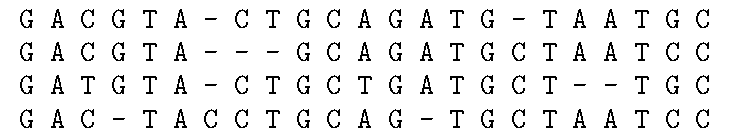
\includegraphics{figures/alignment.pdf}}
\caption{A multiple alignment of four sequences. Character $-$ denotes either a deletion in the current sequence or an insertion in some other sequence.}
\label{fig:multiple alignment}
\end{figure}


\paragraph{Graphs.}

A \emph{graph} $G = (V, E)$ consists of a set $V = \set{v_{1}, \dotsc, 
v_{\abs{V}}}$ of \emph{nodes} and a set $E \subset V^{2}$ of \emph{edges} such that 
$(v, v) \not\in E$ for all $v \in V$. We call $(u, v) \in E$ an edge from node $u$ 
to node $v$. A graph is \emph{directed}, if edge $(u, v)$ is distinct from edge 
$(v, u)$. For every node $v \in V$, 
we define the \emph{indegree} of the node $in(v)$ to be the number of incoming 
edges $(u, v)$, and the \emph{outdegree} $out(v)$ to be the number of outgoing 
edges $(v, w)$.

In a \emph{labeled} graph, we attach a \emph{label} $\ell(v)$ to 
each node $v \in V$. A \emph{path} $\Path = u_{1} \dotsm u_{\abs{\Path}}$ is a sequence of 
nodes such that $(u_{i}, u_{i+1}) \in E$ for all $i 
< \abs{\Path}$. The label of path $\Path$ is the string $\ell(\Path) = \ell(u_{1}) \dotsm 
\ell(u_{\abs{\Path}})$. A \emph{cycle} is a path from a node to itself containing at 
least one other node. If a graph contains no cycles, it is called \emph{acyclic}.

A \emph{tree} is an undirected graph $G = (V, E)$ with exactly one path between any pair of nodes $u, v \in V$. In a \emph{rooted} tree, one node $v_{r} \in V$  is selected as the \emph{root} node. For any edge $(u, v) \in E$, where node $u$ is on the path from root to node $v$, we call node $u$ the \emph{parent} of node $v$, and node $v$ a \emph{child} of node $u$. An \emph{internal} node is a node with children, while a \emph{leaf} node is a node without children.

A \emph{trie} is a rooted tree, where every edge $e \in E$ is labeled by a character $\ell(e) \in \Sigma$. For any internal node $v$, the edges leading to its children must have distinct labels. A path $\Path = e_{1} \dotsm e_{\abs{P}}$ from the root node to a leaf node is labeled by a string $\ell(\Path) = \ell(e_{1}) \dotsm \ell(e_{\abs{\Path}})$. The set of strings $L(G)$ contained in trie $G$ is the set of all path labels from the root to a leaf.

\paragraph{Automata and languages.}

A \emph{finite automaton} is a directed labeled graph $A = (V, E)$.\footnote{Unlike the usual definition, we label nodes instead of edges.} The \emph{initial node} $v_{1}$ is labeled with $\ell(v_{1}) = \#$ with lexicographic value $\sigma + 1$, while the \emph{final node} $v_{\abs{V}}$ is labeled with $\ell(v_{\abs{V}}) = \$$. The rest of the nodes are labeled with characters from alphabet $\Sigma$. We assume that every node $v \in V$ is contained in some path from $v_{1}$ to $v_{\abs{V}}$.

\newpage The \emph{language} $L(A)$ \emph{recognized} by automaton $A$ is the set of all path labels
from $v_{1}$ to $v_{\abs{V}}$. We say that automaton $A$ recognizes any string $S \in L(A)$, and that a suffix $S'$ can be recognized from node $v$, if there is a path from $v$ to $v_{\abs{V}}$ with label $S'$. Note that all strings in the language are 
of form $\# x \$$, where $x$ is a string over alphabet $\Sigma$. If the language 
contains a finite number of strings, it is called \emph{finite}. A language is 
finite if and only if the automaton recognizing it is acyclic. Two automata are said to be \emph{equivalent}, if they recognize the same language.

Automaton $A$ is forward (reverse) \emph{deterministic} if, for every node $v \in V$ and every character $c \in \Sigma \cup \set{\#, \$}$, there exists at most one node $u$ such that $\ell(u) = c$ and $(v, u) \in E$ ($(u, v) \in E$). For any language recognized by some finite automaton, we can always construct an equivalent automaton that is forward (reverse) deterministic.


\section{Full-text indexes}\label{sect:full-text indexes}

Traditional indexes such as the \emph{inverted index} treat the text as a sequence of words. Because of this limitation, they can only support queries based on words or their prefixes efficiently. If the text cannot be split into words, or if we want to search for arbitrary substrings, we must use \emph{full-text indexes} instead. In later chapters, when we need to differentiate between the indexes of different texts, we put the original text or collection into subscript (e.g. $\BWT_{T}$ or $\SA_{\mathcal{C}}$).

\paragraph{Suffix tree and suffix array.}

The suffix trie of text $T[1,n]$ is a trie containing all suffixes of the text. As there are $\Theta(n^{2})$ nodes in the worst case, the suffix trie is not a practical index for large texts. We get the \emph{suffix tree (ST)} \cite{Weiner1973} by replacing every unary path $\Path$ of the trie with a single edge $e$ with label $\ell(e) = \ell(\Path)$. As there is one leaf node for each of the $n$ suffixes and no unary internal nodes, there are at most $2n-1$ nodes. If we store the edge labels as pointers to the text, we can store the suffix tree in $O(n \log n)$ bits. In practice, the size of a suffix tree is usually 10--20 bytes per character \cite{Kurtz1999}. The suffix tree can be constructed in linear time with negligible working space in addition to the text and the final index \cite{McCreight1976,Ukkonen1995}. Given a \emph{pattern} of length $\abs{P}$, we can find the subtree containing its occurrences by following the edge labels in $O(\abs{P})$ time (assuming a constant-sized alphabet). If there are $occ$ occurrences, we can list their positions in the text by traversing the subtree in $O(occ)$ time. An example of the suffix tree and some related indexes can be seen in Figure~\ref{fig:suffix structures}.

\begin{figure}
\centerline{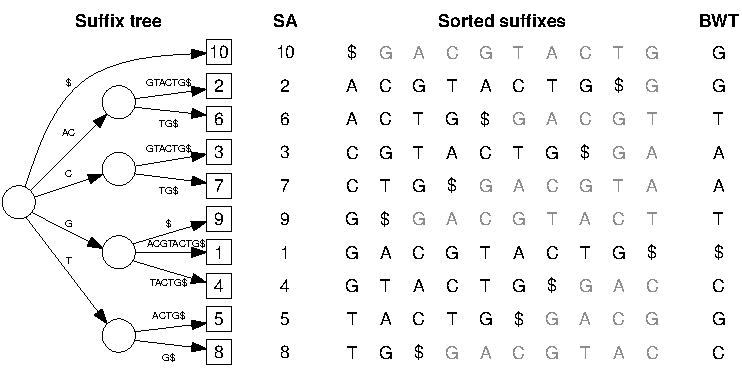
\includegraphics{figures/indexes.pdf}}
\caption{Suffix tree, suffix array, and the Burrows-Wheeler transform of text \texttt{GACGTACTG\$}.}
\label{fig:suffix structures}
\end{figure}

\newpage The \emph{suffix array (SA)} \cite{Manber1993,Gonnet1992} of text $T[1,n]$ is an array of pointers $\SA[1,n]$ to the suffixes of $T$ in lexicographic order. Alternatively, the suffix array is the set of the leaves of the suffix tree, listed according to the lexicographic order of the path labels from root to leaf. The suffix array for text $T[1,n]$ requires $n \log n$ bits of space in addition to the text, and can be constructed in $O(n)$ time with $2n$ bits of working space in addition to the text and the final index \cite{Nong2009}. Given pattern $P$, we can find the range $\SA[sp,ep]$ containing the suffixes that have the pattern as their prefix in $O(\abs{P} \log n)$ by using binary search. Other operations can be supported, but in general the suffix array is more limited than the suffix tree.

\begin{definition}\label{def:suffix array}
A data structure provides suffix array-like functionality, if it supports the following queries efficiently: (a) \find\ the suffix array range $\SA[sp,ep]$ containing the suffixes prefixed by pattern $P$; (b) given $i$, \locate\ suffix $\SA[i]$ in the text; and (c) given $i$ and $j$, \extract\ substring $T[i,j]$.
\end{definition}

An alternate definition for \locate\ is to locate all occurrences of a pattern in the text. This definition is more useful for discussing indexes that are not based on the suffix array, such as the \lzindex{} (see Section~\ref{sect:original indexes}). With these indexes, \find\ is not a meaningful operation, and should be replaced by counting the number of occurrences of a pattern in the text, or just by determining whether there are any occurrences at all.

The suffix tree and the suffix array can be easily \emph{generalized} to handle multiple sequences. Assume we are given a \emph{collection} (a set) of texts $T_{1}, \dotsc, T_{r}$, and let $\$_{i}$ be the end marker of text $T_{i}$. To have strict lexicographic ordering between the suffixes, we define $\$_{i} < \$_{j}$ whenever $i < j$. The generalized suffix trie is now simply a trie containing all suffixes of texts $T_{1}, \dotsc, T_{r}$. Generalized versions of the suffix tree and the suffix array are derived from the trie in the same way as above.

\paragraph{Burrows-Wheeler transform.}

\emph{Burrows-Wheeler transform (BWT)} \cite{Burrows1994} is a permutation of the text closely related to the suffix array. The BWT of text $T[1,n]$ is a sequence $\BWT[1,n]$ such that $\BWT[i] = T[\SA[i] - 1]$, if $\SA[i] > 1$, and $\BWT[i] = T[n] = \$$ otherwise. The transform can be reversed by a permutation called \emph{\LF} \cite{Burrows1994,Ferragina2005a}. Let $C[0,\sigma+1]$ be an array such that $C[c]$ is the number of characters in $\{ \$, 1, 2, \dotsc, c-1 \}$ occurring in the BWT, with $C[0] = C[\$] = 0$ and $C[\sigma + 1] = n$. We define \LF\ as $LF(i) = C[\BWT[i]] + \mrank_{\BWT[i]}(\BWT,i)$, where $\mrank_{c}(\BWT,i)$ is the number of occurrences of character $c$ in prefix $\BWT[1,i]$.

The $\mrank_{\BWT[i]}(\BWT,i)$ in the definition can be interpreted as the lexicographic rank of suffix $T[\SA[i], n]$ among those suffixes preceded by character $\BWT[i]$. Hence $LF(i)$ is the lexicographic rank of suffix $T[\SA[i]-1, n]$ (or $T[n]$, if $\SA[i] = 1$) among all suffixes of the text. This allows us to move from the suffix array position corresponding to suffix $T[\SA[i], n]$ to that of suffix $T[\SA[i]-1, n]$ without using the text or its suffix array.

\begin{figure}
\begin{tabbing}
mm\=mm\=mm\=mm\= \kill
\> \textbf{function} $\operatorname{find}(P)$ \\
\> \> $[sp, ep] \leftarrow [C[P[\abs{P}], C[P[\abs{P}] + 1]]$ \\
\> \> \textbf{for} $i \leftarrow \abs{P}-1$ \textbf{to} $1$ \\
\> \> \> $sp \leftarrow C[P[i]] + \mrank_{P[i]}(\BWT, sp - 1) + 1$ \\
\> \> \> $ep \leftarrow C[P[i]] + \mrank_{P[i]}(\BWT, ep)$ \\
\> \> \> \textbf{if} $[sp, ep] = \emptyset$ \\
\> \> \> \> \textbf{return} $\emptyset$ \\
\> \> \textbf{return} $[sp, ep]$
\end{tabbing}

\caption{Backward searching on Burrows-Wheeler transform \cite{Ferragina2005a}. The body of the loop constitutes one step of backward searching.}\label{fig:backward searching}
\end{figure}

By using \LF, we can support \find\ with just arrays $C$ and $\BWT$ through \emph{backward searching} \cite{Ferragina2005a} (see Figure~\ref{fig:backward searching}). When searching for pattern $P$, the algorithm maintains an invariant that $\SA[sp_{i}, ep_{i}]$ is the range of suffixes prefixed by $P[i,\abs{P}]$. If $\BWT[j]$ and $\BWT[j']$ are the first and the last occurrences of character $P[i-1]$ in range $\BWT[sp_{i}, ep_{i}]$, then $\SA[LF(j), LF(j')]$ is the range of suffixes prefixed by $P[i-1,\abs{P}]$. In Chapter~\ref{chapter:csa}, we show how backward searching can be implemented efficiently in compressed suffix arrays.

\begin{theorem}\label{theorem:backward searching}
Assume that an index performs one step of backward searching in $t_{B}$ time. Then it supports \find$(P)$ in $O(\abs{P} \cdot t_{B})$ time. 
\end{theorem}

The inverse function of \LF\ is $\Psi(i) = \mselect_{c}(\BWT, i - C[c])$, where $c$ is the highest value with $C[c] < i$, and $\mselect_{c}(\BWT,j)$ is the position of the $j$th occurrence of character $c$ in $\BWT$ \cite{Grossi2005}. We will often write $\mchar(i)$ to denote such character $c$. This function allows us to move from the suffix array position of suffix $T[\SA[i], n]$ to that of suffix $T[\SA[i]+1, n]$. Function $\Psi$ is strictly increasing in the range $C_{c} = [C[c] + 1, C[c+1]]$ corresponding to suffixes starting with character $c \in \Sigma$. Note that $T[\SA[i]] = c$ and $\BWT[\Psi(i)] = c$ for every $i \in C_{c}$.

\paragraph{Enhanced suffix array.}

Let $\lcp(A, B)$ be the length of the longest common prefix of sequences $A$ and $B$. The \emph{longest common prefix (LCP) array} of text $T[1,n]$ is an array $\LCP[1,n]$ such that $\LCP[1] = 0$ and $\LCP[i] = \lcp(T[\SA[i-1],n], T[\SA[i],n])$ for $i > 1$. The array requires $n \log n$ bits of space, and can be constructed in $O(n)$ time \cite{Kasai2001,Puglisi2008,Kaerkkaeinen2009,Gog2011,Fischer2011}. The best construction algorithms require little more space than for the text, the suffix array, and the LCP array. By using another $n \log n$-bit array derived from the LCP array, the time complexity of searching for pattern $P$ in a suffix array is reduced from $O(\abs{P} \log n)$ to $O(\abs{P} + \log n)$ \cite{Manber1993}.

The suffix array, the BWT, and the LCP array can be further augmented with various partial representations of suffix tree topology. This approach, generally known as the \emph{enhanced suffix array} \cite{Abouelhoda2004}, allows us to simulate the suffix tree in the same asymptotic time, while using less space. Many compressed suffix tree proposals are based on a similar idea (see Chapter~\ref{chapter:lcp}).


\section{Compressed data structures}\label{sect:compression}

\paragraph{Data structure compression.}

The field of lossless data compression is centered on finding smaller representations for different types of data. Its three main goals are i) compression efficiency, ii) resources required for compressing the data, and iii) resources required for decompression. The relative importance of these goals varies greatly by the applications considered.

In data structure compression, we are not interested in just compressing the data, but we also want to support various operations on the data. Hence the third goal becomes an efficient support for these operations instead of just the efficiency of full decompression. The main tools used are compression methods that support partial decompression, and space-efficient indexes that allow us to quickly find the right part to decompress.

Most data structures contain no extra information in addition to the data they represent. For example, while the suffix array for text $T[1,n]$ requires $n \log n$ bits of space, we can construct it from the text requiring only $n \log \sigma$ bits of space. Hence it should be possible to represent the suffix array in roughly $n \log \sigma$ bits of space. A data structure that achieves this goal while providing efficient support for the required operations is called \emph{succinct}. More generally, a data structure for data $D$ is succinct, if it takes $\abs{D}(1+o(1))$ bits of space, where $\abs{D}$ is the size of data in \emph{bits}, and efficiently supports the required operations.

\emph{Compressed data structures} are still more powerful than succinct ones. Let $H$ be a \emph{complexity metric} that measures the repetitiveness of the data with respect to some model, and let $f$ be a function such that input data $D$ can be compressed into $f(H(D), \abs{D})$ bits. Then a data structure is compressed with respect to metric $H$, if it requires $O(f(H(D), \abs{D}))$ bits of space, and supports the required operations efficiently. Later in this section, we discuss two complexity metrics for textual data: empirical entropy and the number of equal letter runs in the Burrows-Wheeler transform.

We call a succinct or compressed full-text index a \emph{self-index}, if it does not require the original text to operate, and is able to fully reproduce the text. This allows us to replace the original text with the self-index that often requires less space.

\paragraph{Empirical entropy.}

The \emph{empirical entropy} \cite{Manzini2001} $H_{k}(S)$ of sequence $S[1,n]$ is the average uncertainty over the next character in the sequence, given a \emph{context} of $k \ge 0$ previous characters. If we encode each character in the sequence separately, while considering only the $k$ preceding characters during the encoding, then $nH_{k}(S)$ bits is a lower bound for the size of the compressed representation.

\Orderk{0} empirical entropy is defined as
$$
H_{0}(S) = - \sum_{c=1}^{\sigma} \frac{n_{c}}{\abs{S}} \log \frac{n_{c}}{\abs{S}},
$$
where $n_{c}$ is the number of occurrences of character $c$ in sequence $S$, and $0 \log 0 = 0$. For $k > 0$, let $w \in \Sigma^{k}$ be a sequence, and let $w_{S}$ be the concatenation of the characters following the occurrences of $w$ in sequence $S$. \Orderk{k} empirical entropy for $k > 0$ is then defined as
$$
H_{k}(S) = \sum_{w \in \Sigma^{k}} \frac{\abs{w_{S}}}{\abs{S}} H_{0}(w_{S}).
$$
For any $k \ge 0$ and any sequence $S$, it holds that
$$
0 \le H_{k+1}(S) \le H_{k}(S) \le \log \sigma.
$$
These definitions can be generalized for the \emph{integer alphabet} $\mathbb{N} = \set{0, 1, \dotsc}$. In the rest of this thesis, we will write $H_{k}$ instead of $H_{k}(S)$, if sequence $S$ is evident from the context.

\paragraph{Runs in Burrows-Wheeler transform.}

While the empirical entropy is a natural statistical metric of the compressibility of a sequence, it does not reflect well the large-scale repetitiveness of the sequence. Consider an arbitrary sequence $S[1,n]$ and its \orderk{k} empirical entropy $H_{k}(S)$ for $k \ll n$. As $H_{k}(SS) \approx H_{k}(S)$, empirical entropy implies that the size of a compressed representation of the concatenation of two copies of sequence $S$ should be about twice that of a single sequence. However, it is evident that we can compress $SS$ to take only a little more space than the compressed representation of sequence $S$.

For sequences with large-scale repetitiveness, we define another complexity metric that is a natural structural property of suffix arrays and related structures. We consider the number of \emph{equal letter runs} in the Burrows-Wheeler transform of the sequence. When a text is repetitive, the characters preceding lexicographically adjacent suffixes are identical with high probability. Hence the number of runs should be small when the text is repetitive.

Let $T[1,n]$ be a text, and let $\BWT$ be its Burrows-Wheeler transform. If $\BWT[i] = \BWT[i+1]$, then positions $i$ and $i+1$ belong to the same run. As $T[\SA[i],n]$ and $T[\SA[i+1],n]$ are lexicographically adjacent suffixes, and $T[\SA[i]-1] = T[\SA[i+1]-1]$, then $T[\SA[LF(i)],n]$ and $T[\SA[LF(i+1)],n]$ must also be lexicographically adjacent, and hence $LF(i) = LF(i+1) - 1$. This means that, for every run $\BWT[i, i+l-1]$, there is a corresponding \emph{self-repetition} $\SA[i', i'+l-1]$ in the suffix array, with $\SA[i+j] = \SA[i'+j]+1$ for $0 \le j \le l-1$.

Let $R(T)$ be the number of equal letter runs in the BWT of text $T[1,n]$. If the text is evident from the context, we write $R$ instead of $R(T)$. In addition to the trivial upper bound $R \le n$, another bound \cite{Maekinen2005}
$$
R \le n H_{k}(T') + \sigma^{k} \quad \textrm{for all} \, k \ge 0,
$$
where $T'$ is the reverse of text $T$, is also relevant for low-entropy texts.\footnote{The term $\sigma^{k}$ is actually an upper bound for the number of different \orderk{k} contexts appearing in the reverse text.} See Section~\ref{sect:runs} for bounds for the number of runs in texts with large-scale repetitiveness.

\paragraph{Encoding integers.}

Many compression algorithms transform the data into a sequence of integers. These integers are then encoded into \emph{binary strings} with a variety of methods, and the resulting strings are concatenated to form the compressed representation. Encoding scheme $g \colon \mathbb{N} \to \set{0, 1}^{\ast}$ is \emph{prefix-free}, if for any integers $i, j \in \mathbb{N}$, neither of the codes $g(i)$ and $g(j)$ is a prefix of the other. If the encoding scheme is prefix-free, then the compressed sequence can be decoded unambiguously one integer at a time.

\emph{Huffman codes} \cite{Huffman1952} are based on binary trees. Initially, each integer $i \in \mathbb{N}$ with $n_{i} > 0$ occurrences forms a separate tree with one node. As long as there are multiple trees left, we select two trees $G_{1}$ and $G_{2}$ with the least number of occurrences $n(G_{1})$ and $n(G_{2})$, and replace them with a new tree $G$ with $n(G) = n(G_{1}) + n(G_{2})$ occurrences. Tree $G$ consists of a root node with $G_{1}$ as its left subtree and $G_{2}$ as its right subtree. The final tree is a \emph{Huffman tree} for frequencies $(n_{i})_{i \in \mathbb{N}}$.

To read the codes from the Huffman tree, we label each edge from a node to its left child with $0$, and each edge to right child with $1$. The code for integer $i$ corresponding to leaf node $v_{i}$ is then the path label from root to node $v_{i}$. With the help of a lookup table, both encoding and decoding can be done in constant time per symbol. 

Huffman codes are prefix-free and optimal among those prefix-free codes that encode each occurrence of an integer with the same binary string \cite{Huffman1952}. The average code length is less than $H_{0} + 1$ bits per symbol. Assuming that the integers are bounded by some polynomial $poly(n)$, where $n$ is the length of the sequence, we can compress the sequence into $n(H_{0} + 1) + O(\sigma \log n)$ bits, where $\sigma$ is the number of integers with a positive number of occurrences. The $O(\sigma \log n)$ term comes from storing the number of occurrences for each of the occurring integers.

\emph{Elias codes} \cite{Elias1975} assign fixed codes to all positive integers. They are useful in situations, where the distribution is not known at the time of encoding, or when storing the numbers of occurrences would require significant space. The implicit assumption behind Elias codes is that small integers are more common than large ones, which is often true in e.g. encoding the differences of an increasing sequence of integers.

\newpage Let $b(i)$ be the length $\abs{b(i)} = \lceil \log (i+1) \rceil$ binary representation of integer $i > 0$, and let $b'(i)$ be the same sequence without the leading \onebit. The Elias \emph{\gammacode} for integer $i$ is the binary string $\gamma(i) = 0^{\abs{b'(i)}}  b(i)$ of length $2\abs{b(i)} - 1$. These codes are prefix-free, and encoding and decoding them takes constant time with the help of a lookup table. If we replace the unary representation $0^{\abs{b'(i)}}$ with another \gammacode, we get \emph{\deltacode{}s} $\delta(i) = \gamma(\abs{b(i)}) b'(i)$ of length $\log i + O(\log \log i)$. In general, \gammacode{}s are better when most of the integers are small, while \deltacode{}s require asymptotically less space (see also Section~\ref{sect:bit vectors}).

For an example, consider a simple \emph{run-length encoding} of the BWT of text $T[1,n]$. For a run consisting of $l$ occurrences of character $c$, we output a pair of integers $(c, l)$. The character is encoded directly using $\lceil \log \sigma \rceil$ bits, while \deltacode{}s are used for encoding the length of the run. As logarithm is a concave function, the worst case for encoding a given number of runs is when all the runs are of similar length. For $R$ runs, the average length of a run is $n / R$ characters, so the encoding uses at most
$$
R (\log \sigma + \log (n / R)) + O(R \log \log (n / R))
$$
bits of space. See Section~\ref{sect:rlcsa analysis} for the size bound for another variant of run-length encoding.
